\documentclass[12pt,a4paper]{article}

\usepackage[utf8]{inputenc}
\usepackage[T1]{fontenc}
\usepackage{lmodern}
\usepackage[margin=2.45cm]{geometry}
\usepackage{microtype}
\usepackage{setspace}
\usepackage{parskip}
\usepackage{amsmath,amssymb}
\usepackage{booktabs}
\usepackage{array}
\usepackage{longtable}
\usepackage{tabularx}
\usepackage{xcolor}
\usepackage{hyperref}
\usepackage{enumitem}
\usepackage{listings}
\usepackage{tikz}
\usepackage{fancyhdr}
\usepackage{titlesec}
\usepackage{caption}
\usetikzlibrary{positioning}

\definecolor{insatblue}{HTML}{12355B}
\definecolor{insatteal}{HTML}{1D7874}
\definecolor{softgray}{HTML}{F4F6F8}
\definecolor{codegray}{HTML}{2D3748}
\definecolor{rulegray}{HTML}{D6DEE6}

\hypersetup{
    colorlinks=true,
    linkcolor=insatblue,
    urlcolor=insatteal,
    citecolor=insatblue,
    pdfauthor={INSAT Logic Programming Project},
    pdftitle={Intelligent Energy-Aware Campus Resource Scheduling System}
}

\pagestyle{fancy}
\fancyhf{}
\lhead{\textit{Intelligent Campus Scheduling}}
\rhead{\textit{Logic Programming}}
\cfoot{\thepage}
\renewcommand{\headrulewidth}{0.4pt}
\renewcommand{\headrule}{\hbox to\headwidth{\color{rulegray}\leaders\hrule height \headrulewidth\hfill}}

\titleformat{\section}
  {\Large\bfseries\color{insatblue}}
  {\thesection}{0.8em}{}
\titleformat{\subsection}
  {\large\bfseries\color{insatteal}}
  {\thesubsection}{0.8em}{}
\titleformat{\subsubsection}
  {\normalsize\bfseries\color{codegray}}
  {\thesubsubsection}{0.8em}{}

\lstdefinelanguage{Prolog}{
    morekeywords={
        module,use_module,member,findall,forall,format,write,nl,is,
        fail,true,not,catch,halt,initialization
    },
    sensitive=true,
    morecomment=[l]\%,
    morestring=[b]',
    morestring=[b]"
}
\lstdefinelanguage{PlainText}{}

\lstset{
    language=Prolog,
    basicstyle=\ttfamily\small\color{codegray},
    keywordstyle=\bfseries\color{insatblue},
    commentstyle=\itshape\color{gray},
    stringstyle=\color{insatteal},
    backgroundcolor=\color{softgray},
    frame=single,
    rulecolor=\color{rulegray},
    breaklines=true,
    columns=fullflexible,
    keepspaces=true,
    showstringspaces=false,
    tabsize=2,
    captionpos=b
}

\setstretch{1.12}
\setlist[itemize]{topsep=4pt,itemsep=2pt,parsep=0pt}
\setlist[enumerate]{topsep=4pt,itemsep=2pt,parsep=0pt}

\newcommand{\predicate}[1]{\texttt{#1}}
\newcommand{\term}[1]{\texttt{#1}}
\newcommand{\kw}[1]{\textbf{#1}}

\begin{document}

\begin{titlepage}
    \centering
    \vspace*{1.2cm}
    {\Large\bfseries Institut National des Sciences Appliquees et de Technologie\par}
    \vspace{0.35cm}
    {\large INSAT\par}
    \vspace{1.8cm}
    {\color{insatblue}\rule{0.86\textwidth}{1.2pt}\par}
    \vspace{0.8cm}
    {\Huge\bfseries\color{insatblue} Intelligent Energy-Aware Campus Resource Scheduling System\par}
    \vspace{0.35cm}
    {\Large Declarative Scheduling in SWI-Prolog\par}
    \vspace{0.8cm}
    {\color{insatblue}\rule{0.86\textwidth}{1.2pt}\par}
    \vspace{1.5cm}
    \begin{tabular}{>{\bfseries}rl}
        Course: & Logic Programming \\
        Term: & Spring 2026 \\
        Institution: & INSAT \\
        Implementation Language: & SWI-Prolog \\
        Project Type: & Constraint reasoning and optimization \\
    \end{tabular}
    \vfill
    {\large Final Project Report\par}
    \vspace{0.35cm}
    {\large May 2026\par}
\end{titlepage}

\tableofcontents
\newpage

\section{Abstract}

This report documents the design and implementation of an intelligent, energy-aware campus resource scheduling system for INSAT. The system models the weekly timetable generation problem as a declarative constraint satisfaction and optimization task in SWI-Prolog. Courses, student groups, rooms, instructors, buildings, and time slots are represented as logical facts, while feasibility rules are expressed through predicates that enforce room availability, group availability, room capacity, equipment compatibility, instructor availability, and building-level energy thresholds.

The project goes beyond producing any valid timetable. It integrates symbolic search with quantitative reasoning by computing per-assignment energy consumption, daily building energy usage, total weekly energy, daily load imbalance, and room allocation fairness. A recursive generator constructs schedules incrementally and applies constraints immediately so that impossible branches fail before they expand. Optimization is handled by collecting a bounded number of valid schedules using \predicate{findnsols/4}, then ranking the candidates through a composite score combining total energy, daily imbalance, and room fairness penalties. The result is a modular Prolog decision engine that demonstrates how declarative logic can express and solve a realistic university resource allocation problem.

\section{Introduction}

University timetable generation is a classical operations research problem. It requires assigning many academic sessions to limited physical and temporal resources while respecting institutional, pedagogical, and logistical constraints. The difficulty is not only that many choices exist, but that choices interact: assigning one course to a room at a given time affects room availability, group availability, instructor availability, energy consumption, and the feasibility of later assignments.

Logic programming is particularly well suited to this type of problem because it separates the statement of constraints from the operational mechanism used to search through possible solutions. In Prolog, a timetable can be described as a set of terms, and the validity of that timetable can be described as relations over those terms. Backtracking then provides a natural search mechanism. The programmer states what makes an assignment valid, and Prolog explores alternatives until a consistent structure is found.

The implemented system, named \emph{Intelligent Energy-Aware Campus Resource Scheduling System}, applies this idea to a representative INSAT campus model. It schedules courses over a six-day academic week, with five time slots per day, using approximately 130 modeled rooms distributed over three energy zones. The project also introduces energy-aware reasoning: each room has an hourly consumption rate, each slot lasts 1.5 hours, and each building wing has a daily energy threshold. Therefore, the scheduler must respect not only classroom and pedagogical constraints, but also physical operating limits.

\section{Problem Statement and Modeling}

\subsection{Formal Scheduling Problem}

Let \(C\) denote the set of courses, \(G\) the set of student groups, \(R\) the set of rooms, \(T\) the set of time slots, and \(B\) the set of building zones. The objective is to assign each required course session to exactly one room and one time slot:

\[
    f : (C \times G) \rightarrow (R \times T)
\]

subject to hard constraints:

\begin{enumerate}
    \item No room may host two sessions in the same slot.
    \item No student group may attend two sessions in the same slot.
    \item The room capacity must be greater than or equal to the group enrollment.
    \item The room equipment must satisfy the course equipment requirement.
    \item The course instructor must be available in the selected slot.
    \item The daily energy consumption of the selected building must not exceed its threshold.
\end{enumerate}

The system must also compare valid schedules according to soft optimization criteria: total energy consumption, daily load balance, and fairness of room usage.

\subsection{Logical Representation}

The central assignment structure is:

\begin{lstlisting}[caption={Assignment term used throughout the scheduler}]
assign(CourseID, GroupID, RoomID, slot(Day, Index))
\end{lstlisting}

This representation is compact but expressive. It binds the four essential dimensions of the scheduling problem: a course, the group attending it, the room where it occurs, and the temporal slot in which it is placed. Since assignments are ordinary Prolog terms, schedules can be represented as recursive lists:

\begin{lstlisting}[caption={Schedule as a recursive list of assignment terms}]
[
  assign(gl3_lp_lec, gl3_a, amphi_a1, slot(monday, 1)),
  assign(gl3_lp_tp,  gl3_a, r136,     slot(monday, 4))
]
\end{lstlisting}

The knowledge base is divided into domain-specific modules. This modularity keeps static institutional facts separate from derived constraints and optimization rules.

\begin{table}[h]
    \centering
    \caption{Main Prolog modules}
    \begin{tabularx}{\textwidth}{>{\ttfamily}lX}
        \toprule
        Module & Responsibility \\
        \midrule
        courses.pl & Course facts, sessions per week, required equipment, instructor association, and course-group mappings. \\
        groups.pl & Student group identifiers, departments, years, and enrollment sizes. \\
        buildings\_and\_rooms.pl & Building zones, room facts, capacities, equipment types, and room energy rates. \\
        instructors.pl & Instructor facts and closed-world availability exceptions. \\
        time\_slots.pl & Six academic days, five daily slots, and 1.5-hour slot duration. \\
        constraints.pl & Hard feasibility predicates for capacity, equipment, instructor availability, and conflicts. \\
        energy.pl & Energy computation and building daily threshold checking. \\
        generator.pl & Recursive schedule construction and bounded schedule enumeration. \\
        optimizer.pl & Composite schedule scoring and best-schedule selection. \\
        interface.pl & User-facing orchestration and terminal display. \\
        config.pl & Scenario selection, candidate limits, optimization mode, and energy flag. \\
        \bottomrule
    \end{tabularx}
\end{table}

\subsection{Knowledge Base Scale}

The implemented model contains 130 rooms, 146 course facts, 79 student groups, 30 weekly time slots, 62 instructors, and 3 building energy zones. The room model includes amphitheaters, standard lecture rooms, computer science laboratories, physics laboratories, chemistry laboratories, biology laboratories, electronics laboratories, language laboratories, and a central auditorium. The temporal model contains six days from Monday to Saturday and five 1.5-hour slots per day, producing \(6 \times 5 = 30\) possible weekly slots.

\begin{table}[h]
    \centering
    \caption{Knowledge base size verified from the implementation}
    \begin{tabular}{lr}
        \toprule
        Entity & Count \\
        \midrule
        Rooms & 130 \\
        Building energy zones & 3 \\
        Courses & 146 \\
        Student groups & 79 \\
        Instructors & 62 \\
        Weekly time slots & 30 \\
        \bottomrule
    \end{tabular}
\end{table}

\section{System Architecture}

The scheduler follows a layered architecture. The lowest layer is the knowledge base, which contains declarative facts. The middle layer contains the reasoning predicates: hard constraints, energy accumulation, and recursive generation. The upper layer contains optimization and interfaces.

\begin{figure}[h]
    \centering
    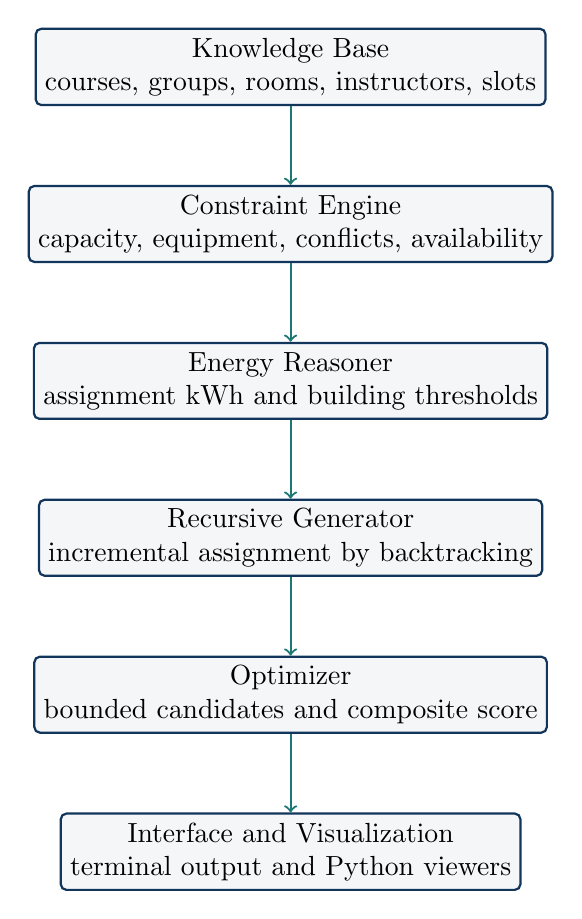
\begin{tikzpicture}[
        node distance=1.0cm,
        block/.style={rectangle, rounded corners=2pt, draw=insatblue, thick, fill=softgray, align=center, minimum width=4.2cm, minimum height=0.85cm},
        arrow/.style={->, thick, color=insatteal}
    ]
        \node[block] (kb) {Knowledge Base\\courses, groups, rooms, instructors, slots};
        \node[block, below=of kb] (constraints) {Constraint Engine\\capacity, equipment, conflicts, availability};
        \node[block, below=of constraints] (energy) {Energy Reasoner\\assignment kWh and building thresholds};
        \node[block, below=of energy] (generator) {Recursive Generator\\incremental assignment by backtracking};
        \node[block, below=of generator] (optimizer) {Optimizer\\bounded candidates and composite score};
        \node[block, below=of optimizer] (ui) {Interface and Visualization\\terminal output and Python viewers};

        \draw[arrow] (kb) -- (constraints);
        \draw[arrow] (constraints) -- (energy);
        \draw[arrow] (energy) -- (generator);
        \draw[arrow] (generator) -- (optimizer);
        \draw[arrow] (optimizer) -- (ui);
    \end{tikzpicture}
    \caption{Layered architecture of the scheduling system}
\end{figure}

The entry point \predicate{main.pl} loads the modules in dependency order. Runtime settings are centralized in \predicate{config.pl}; therefore, switching from a small demonstration scenario to a larger engineering or full-campus scenario does not require changing the scheduler logic. The configuration supports environment variables such as \term{SCHED\_SCENARIO}, \term{SCHED\_LIMIT}, \term{SCHED\_OPT}, and \term{SCHED\_ENERGY}.

\section{Constraint Engine and Search Complexity}

\subsection{Hard Constraint Predicates}

The constraint engine in \predicate{constraints.pl} implements the hard feasibility conditions required by the project. The main exported predicates are:

\begin{itemize}
    \item \predicate{equipment\_satisfied/2}: verifies that a room's equipment type satisfies the course requirement.
    \item \predicate{capacity\_satisfied/3}: verifies that the room can contain the target group.
    \item \predicate{instructor\_available\_for/2}: checks that the assigned instructor is available for the proposed slot.
    \item \predicate{no\_room\_conflict/1}: validates that no two assignments use the same room at the same time.
    \item \predicate{no\_group\_conflict/1}: validates that no group is scheduled in two places at once.
    \item \predicate{all\_constraints\_satisfied/2}: combines the incremental checks for one new assignment against the current partial schedule.
\end{itemize}

The combined incremental predicate is the critical entry point used by the generator:

\begin{lstlisting}[caption={Incremental constraint checking order}]
all_constraints_satisfied(assign(C, G, R, Slot), Existing) :-
    equipment_satisfied(C, R),
    capacity_satisfied(C, G, R),
    instructor_available_for(C, Slot),
    room_free_for(R, Slot, Existing),
    group_free_at(G, Slot, Existing).
\end{lstlisting}

This predicate expresses an important engineering decision: constraints are ordered from cheapest and most discriminating to more expensive list-scanning checks.

\subsection{Constraint Ordering and Early Failure}

The difference between efficient test-and-generate and inefficient generate-and-test is central to the project. A naive implementation could generate a complete schedule first and then ask whether it satisfies all constraints. Such a design would waste most of its time constructing invalid structures. In contrast, this implementation checks every candidate assignment before appending it to the partial schedule.

The order of checks is deliberate:

\begin{enumerate}
    \item \predicate{equipment\_satisfied/2} is a static fact lookup using \predicate{course/8}, \predicate{room/6}, and \predicate{equipment\_compatible/2}.
    \item \predicate{capacity\_satisfied/3} is another static lookup comparing group enrollment and room capacity.
    \item \predicate{instructor\_available\_for/2} uses the closed-world availability model: an instructor is available unless explicitly listed as unavailable.
    \item \predicate{room\_free\_for/3} scans the existing partial schedule.
    \item \predicate{group\_free\_at/3} scans the existing partial schedule.
\end{enumerate}

The first three checks are essentially constant-time knowledge base lookups for a given candidate. They do not traverse the partial schedule. The room and group conflict checks are \(O(n)\), where \(n\) is the number of assignments already placed. Placing the \(O(1)\) checks first prevents expensive scans for candidates that are impossible for simpler reasons, such as a chemistry practical session being proposed in a standard lecture room or a group being placed in a room whose capacity is below its enrollment.

\subsection{Theoretical Branching Factor}

For a single session, the unconstrained choice is:

\[
    |\text{Rooms}| \times |\text{Slots}| = 130 \times 30 = 3900
\]

Thus, a random assignment procedure has a theoretical branching factor of approximately 3900 choices per session. If \(N\) sessions must be scheduled, the naive search space is on the order of \(3900^N\), before considering conflicts and instructor constraints. This is computationally infeasible even for moderate \(N\).

Early-failure constraints reduce this branching factor immediately. For example, a physics laboratory session requires \term{physics\_lab}. The model contains 10 physics laboratories: five on floor 1 and five on floor 2. Therefore, before checking time conflicts, equipment compatibility reduces the room dimension from 130 to 10. The branch count for that class of session falls from:

\[
    130 \times 30 = 3900
\]

to approximately:

\[
    10 \times 30 = 300
\]

This is a reduction of more than 92\% before capacity, instructor availability, room occupancy, group occupancy, or energy constraints are applied. Similar reductions occur for computer science laboratories, chemistry laboratories, biology laboratories, electronics laboratories, language laboratories, and amphitheater-based lectures.

\subsection{Incompleteness and Inefficiency Risks}

The system becomes inefficient if constraints are delayed until after complete schedule generation. In that case, Prolog would recursively enumerate assignments whose invalidity could have been detected earlier. The system also becomes inefficient if expensive list-scanning predicates are called before static compatibility checks.

Incompleteness can arise from modeling choices rather than from Prolog itself. If the knowledge base gives a course an equipment requirement for which no room exists, or if all compatible rooms are too small for a required group, the search correctly fails. During validation, this risk was addressed by adding an integration test requiring every declared \predicate{course\_session/2} to have at least one feasible room. Similarly, if energy thresholds are set unrealistically low, otherwise feasible academic schedules may be rejected. Such failure is logically correct relative to the model, but it indicates that institutional data or thresholds must be reviewed.

\section{Recursive Generation}

\subsection{Work List Construction}

The generator in \predicate{generator.pl} first builds a work list from the active scenario. The predicate \predicate{scenario\_courses/1} selects courses according to department and year, while \predicate{scenario\_groups/1} selects the corresponding student groups. The facts \predicate{course\_session/2} determine which groups attend each course. Since courses may require one or two sessions per week, \predicate{expand\_sessions/2} expands each course-group pair into repeated \term{work\_item(C,G)} terms.

After expansion, the work list is ordered by difficulty. Each \term{work\_item(C,G)} is keyed by the number of rooms that satisfy both \predicate{equipment\_satisfied/2} and \predicate{capacity\_satisfied/3}. Sessions with fewer compatible rooms are scheduled first. This is a fail-first heuristic: laboratory sessions and high-capacity requirements are handled before flexible lecture sessions, which substantially improves larger scenarios because infeasible branches are detected near the top of the search tree.

\begin{lstlisting}[caption={Recursive assignment structure}]
generate_schedule(Assignments) :-
    build_work_list(WorkList),
    assign_all(WorkList, [], Assignments).

assign_all([], Acc, Acc).
assign_all([work_item(C, G) | Rest], Partial, Final) :-
    assign_one(C, G, Partial, NewAssign),
    assign_all(Rest, [NewAssign | Partial], Final).
\end{lstlisting}

The base case returns the accumulated schedule once all work items have been placed. The recursive case assigns one session, checks it against the partial schedule, and continues with the rest.

\subsection{Backtracking over Rooms and Slots}

For each work item, \predicate{assign\_one/4} enumerates candidate slots and rooms through Prolog backtracking:

\begin{lstlisting}[caption={Candidate generation and immediate validation}]
assign_one(CourseID, GroupID, Partial,
           assign(CourseID, GroupID, RoomID, Slot)) :-
    time_slot(Slot, _Day, _SH, _SM, _EH, _EM),
    room(RoomID, _Building, _Floor, _Cap, _Equip, _ERate),
    Candidate = assign(CourseID, GroupID, RoomID, Slot),
    all_constraints_satisfied(Candidate, Partial),
    check_energy_constraint(Candidate, Partial).
\end{lstlisting}

The generator therefore has a clear declarative reading: choose a time slot, choose a room, form an assignment, and accept it only if all symbolic and energy constraints hold. If a candidate fails, Prolog automatically backtracks to another room or slot.

\section{Energy Modeling}

\subsection{Energy Facts and Physical Interpretation}

Energy reasoning is implemented in \predicate{energy.pl}. Each room fact includes an hourly energy rate in kilowatts. A standard lecture room is modeled at 3.0 kW, computer science laboratories at 5.5 kW, chemistry laboratories at 6.5 kW, amphitheaters at 6.0 kW, and the auditorium at 15.0 kW. Each slot lasts 1.5 hours, so the energy of one assignment is:

\[
    E_{\text{assignment}} = \text{HourlyRate}_{\text{room}} \times 1.5
\]

This is encoded by \predicate{assignment\_energy/2}:

\begin{lstlisting}[caption={Per-session energy computation}]
assignment_energy(assign(_C, _G, RoomID, _Slot), Energy) :-
    room(RoomID, _Building, _Floor, _Cap, _Equip, HourlyRate),
    slot_duration_hours(Duration),
    Energy is HourlyRate * Duration.
\end{lstlisting}

The campus is logically divided into three building energy zones: \term{insat\_amphi\_wing}, \term{insat\_f1\_wing}, and \term{insat\_f2\_wing}. The amphitheater zone has a daily threshold of 500 kWh, while the first-floor and second-floor wings each have a daily threshold of 900 kWh.

\subsection{Dynamic Threshold Checking}

The key energy predicate is \predicate{building\_energy\_ok/3}. It computes the total energy already assigned to a building on a given day and succeeds only if the total remains below the building threshold:

\begin{lstlisting}[caption={Daily building threshold constraint}]
building_energy_ok(Day, Assignments, Building) :-
    building(Building, _Name, Threshold),
    building_daily_energy(Day, Assignments, Building, Used),
    Used =< Threshold.
\end{lstlisting}

This predicate is called during generation, not only after completion. When a new assignment is proposed, the generator constructs a projected partial schedule containing the new assignment and checks the affected building:

\begin{lstlisting}[caption={Energy check during recursive generation}]
check_energy_constraint(assign(C, G, RoomID, slot(Day, Idx)), Partial) :-
    setting(enable_energy_constraints, Flag),
    (   Flag = false
    ->  true
    ;   room(RoomID, Building, _Floor, _Cap, _Equip, _ERate),
        ProposedList = [assign(C, G, RoomID, slot(Day, Idx)) | Partial],
        building_energy_ok(Day, ProposedList, Building)
    ).
\end{lstlisting}

This design incorporates physical limits into the symbolic search. If adding a session to \term{insat\_f1\_wing} would exceed its daily limit of 900 kWh, the candidate fails immediately and the generator backtracks. Energy is therefore a pruning constraint, not merely a post-processing statistic.

\section{Optimization and Fairness}

\subsection{Avoiding Combinatorial Explosion}

The full-campus scheduling problem has a very large number of valid and invalid configurations. Attempting to enumerate all valid schedules before optimization would be impractical. The project avoids this combinatorial explosion by decoupling schedule generation from schedule ranking.

The generator uses \predicate{findnsols/4} through \predicate{generate\_n\_schedules/2}:

\begin{lstlisting}[caption={Bounded candidate generation}]
generate_n_schedules(N, Schedules) :-
    findnsols(N, S, generate_schedule(S), Schedules).
\end{lstlisting}

Instead of collecting every possible valid schedule, the system collects at most \(N\) schedules, where \(N\) is controlled by \term{SCHED\_LIMIT}. This creates a deterministic and tunable boundary around the optimization stage. Once the candidate subset is available, selecting the best schedule is linear in the number of candidates:

\[
    O(N)
\]

where \(N\) is the configured candidate limit, not the total number of theoretically possible schedules.

\subsection{Composite Scoring Function}

The optimizer reduces each structured schedule to a scalar score:

\[
    \text{Score} =
    \text{TotalEnergy}
    + W_1 \times \text{DailyImbalance}
    + W_2 \times \text{RoomFairnessPenalty}
\]

In the implementation, \(W_1 = 0.5\) and \(W_2 = 0.3\). Lower scores are better:

\begin{lstlisting}[caption={Multi-criteria schedule score}]
schedule_score(Assignments, Score) :-
    total_weekly_energy(Assignments, Energy),
    daily_load_imbalance(Assignments, Imbalance),
    room_fairness_penalty(Assignments, Fairness),
    w_imbalance(W1),
    w_fairness(W2),
    Score is Energy + W1 * Imbalance + W2 * Fairness.
\end{lstlisting}

This scoring function is declarative because it defines a relation between a schedule and a numeric quality value. Once the relation is available, comparing schedules becomes simple numerical comparison rather than nested structural reasoning.

\subsection{Daily Load Imbalance}

Daily load imbalance is computed as the difference between the maximum and minimum active-day energy totals:

\[
    \text{DailyImbalance} =
    \max_{d \in D} E_d - \min_{d \in D} E_d
\]

This metric penalizes schedules that concentrate energy use on one day while leaving other days light. In a real campus, reducing daily peaks is useful because high peaks can stress electrical infrastructure and may correspond to higher operational cost.

\subsection{Room Fairness Penalty}

Room fairness is computed as the variance of per-room assignment counts among rooms used by the schedule. If one or two rooms carry most sessions while other compatible rooms remain unused, the penalty increases. This models concerns such as equipment wear, maintenance load, crowd movement concentration, and uneven use of campus resources.

\subsection{Fairness versus Energy Efficiency}

The energy and fairness objectives conflict. An energy-minimizing schedule tends to compact classes into a small number of rooms or buildings, reducing the number of active zones and preferring lower-energy rooms. A fairness-oriented schedule spreads classes more uniformly across available rooms, which may activate more rooms and building zones and therefore consume more energy. The implemented composite score resolves this conflict through weights. Increasing \(W_1\) emphasizes daily load smoothing; increasing \(W_2\) emphasizes fairer room distribution; reducing both makes total energy dominate.

This weighted-sum approach is appropriate for the project because it is transparent, easy to justify, and compatible with Prolog's symbolic generation. It also keeps optimization modular: the generator does not need to know how schedules are evaluated, and the optimizer does not need to know how schedules are constructed.

\section{Integration and Visualization Interface}

\subsection{Main Orchestration}

The predicate \predicate{run\_scheduler/0}, provided by \predicate{interface.pl}, coordinates the complete reasoning pipeline:

\begin{enumerate}
    \item Read runtime settings from \predicate{config.pl}.
    \item Build the session work list.
    \item Generate a bounded list of valid schedules.
    \item Select the first schedule or the best schedule depending on the optimization mode.
    \item Display the timetable and total weekly energy.
\end{enumerate}

The same code path supports multiple scenarios:

\begin{itemize}
    \item \term{demo}: GL year 3, useful for quick validation.
    \item \term{gl3\_only}: all GL years 2 to 5.
    \item \term{engineering}: engineering departments and years.
    \item \term{full\_campus}: the complete knowledge base.
\end{itemize}

\subsection{Python Viewers}

The project includes two Python visualization tools. \predicate{schedule\_viewer.py} provides an interactive terminal viewer, while \predicate{schedule\_visualizer.py} provides a Tkinter graphical interface. These tools parse Prolog output in the form:

\begin{lstlisting}[caption={Parsed Prolog assignment format}]
assign(CourseID, GroupID, RoomID, slot(Day, SlotIndex))
\end{lstlisting}

They then render schedules by room, by group, by day, as a timetable grid, and as summary statistics. This division of responsibilities is coherent: Prolog remains responsible for logical reasoning, while Python handles user-oriented visualization.

\section{Validation and Execution Results}

\subsection{Sanity and Integration Tests}

The test file verifies that the three main knowledge bases load successfully: groups, rooms, and courses. It also performs integration checks that validate the interaction between modules:

\begin{itemize}
    \item every declared \predicate{course\_session/2} has at least one feasible room satisfying both equipment and capacity;
    \item full-campus scenario selection includes prep-stream courses and prep-stream groups;
    \item the demo scenario can generate a complete schedule;
    \item the generated schedule has no room or group conflicts;
    \item an explicit over-threshold building energy schedule is rejected.
\end{itemize}

The local execution produced:

\begin{lstlisting}[language=PlainText,caption={Sanity test result}]
[test] Groups loaded successfully.
[test] Rooms loaded successfully.
[test] Courses loaded successfully.
[test] Every course/group session has at least one feasible room.
[test] Full-campus prep course/group selection works.
[test] Schedule generation succeeded (32 assignments).
[test] Generated schedule has no room/group conflicts.
[test] Energy threshold violation is rejected.
All sanity tests passed!
\end{lstlisting}

This confirms not only that facts are accessible to SWI-Prolog, but also that the main knowledge bases are mutually consistent. In particular, prep-stream courses use the abstract year \term{prep}, while prep-stream groups are represented as \term{prep1} and \term{prep2}. The scenario manager bridges this vocabulary difference during group selection, so \term{full\_campus} includes both prep courses and prep groups.

\subsection{Demonstration Scenario}

Using the \term{demo} scenario with \term{SCHED\_LIMIT=1}, \term{SCHED\_OPT=balanced}, and enabled energy constraints, the scheduler produced one valid timetable for GL3. The generated work list contained 32 session-items, and the resulting schedule contained 32 assignments. The reported total weekly energy was 285.00 kWh.

\begin{table}[h]
    \centering
    \caption{Verified demo run}
    \begin{tabular}{ll}
        \toprule
        Setting or result & Value \\
        \midrule
        Scenario & \term{demo} \\
        Candidate limit & 1 \\
        Optimization mode & \term{balanced} \\
        Energy constraints & enabled \\
        Work-list size & 32 session-items \\
        Valid schedules found & 1 \\
        Final assignments & 32 \\
        Total weekly energy & 285.00 kWh \\
        \bottomrule
    \end{tabular}
\end{table}

The generated timetable placed GL3 activities from Monday through Thursday, using amphitheaters for lecture and tutorial-style sessions and computer science laboratories for practical sessions. This is consistent with the equipment compatibility rules: courses requiring \term{cs\_lab} are assigned to rooms such as \term{r136} and \term{r137}, while lecture sessions requiring \term{projector\_board} can be placed in amphitheaters because \predicate{equipment\_compatible/2} explicitly allows amphitheaters to satisfy standard projection needs.

\subsection{Experimental Validation}

The following experiments were executed locally with SWI-Prolog 10.0.2. Each run collected the first valid schedule unless otherwise stated. The results show that the system scales from the demonstration scenario to the full-campus scenario after applying fail-first work-list ordering and prep-year normalization in \predicate{config.pl}.

\begin{table}[h]
    \centering
    \caption{Scenario scaling and energy-constraint experiment}
    \begin{tabular}{lrrrrr}
        \toprule
        Scenario & Energy checks & Work items & Found & Energy (kWh) & Time (ms) \\
        \midrule
        \term{demo} & true & 32 & 1 & 285.00 & 33--48 \\
        \term{demo} & false & 32 & 1 & 285.00 & 48 \\
        \term{gl3\_only} & true & 90 & 1 & 798.00 & 152 \\
        \term{engineering} & true & 278 & 1 & 2113.50 & 634 \\
        \term{engineering} & false & 278 & 1 & 2149.50 & 612 \\
        \term{full\_campus} & true & 796 & 1 & 5046.75 & 4141 \\
        \term{full\_campus} & false & 796 & 1 & 5100.75 & 3297 \\
        \bottomrule
    \end{tabular}
\end{table}

The energy constraint did not make these tested scenarios infeasible; the building thresholds are high enough to admit valid timetables. However, the energy-aware search changed the first full-campus and engineering schedules returned by Prolog, reducing the observed weekly energy from 5100.75 kWh to 5046.75 kWh in \term{full\_campus}, and from 2149.50 kWh to 2113.50 kWh in \term{engineering}. This indicates that energy constraints are active during generation, not merely computed afterward.

For optimization validation, the demo scenario was also run with \term{SCHED\_LIMIT=5}. Five valid candidate schedules were collected in 45 ms. The best candidate selected by \predicate{best\_schedule/2} had total energy 285.00 kWh and composite score 331.15. This confirms that the optimizer can compare several valid schedules rather than only displaying the first solution.

\section{Critical Analysis}

\subsection{Why Declarative Modeling Fits the Problem}

The project benefits from Prolog because the central entities are naturally relational. A room has a capacity, a course has an equipment requirement, a group has an enrollment, and a slot has a day and index. Constraints are relations among these facts. For example, capacity satisfaction is not implemented as a procedural loop over objects; it is a logical condition over \predicate{group\_size/2} and \predicate{room/6}. Similarly, instructor availability is a logical condition over instructor facts and unavailability exceptions.

Backtracking is also appropriate because the search problem is inherently nondeterministic. There is no single obvious room or slot for a course before constraints are considered. Prolog's search mechanism allows the system to express alternatives directly and let failed constraints trigger automatic reconsideration.

\subsection{Search Complexity Answer}

Constraint ordering has a direct effect on search complexity. The implementation places \predicate{equipment\_satisfied/2} and \predicate{capacity\_satisfied/3} first because they are static fact checks and reject many impossible room choices immediately. Instructor availability is also checked before scanning the partial schedule. Only after these checks succeed does the engine call list-scanning predicates such as \predicate{room\_free\_for/3} and \predicate{group\_free\_at/3}.

This ordering turns many failures into cheap failures. A candidate assignment that violates equipment requirements fails before the partial schedule is traversed. A candidate that violates capacity fails before room and group conflicts are examined. Since these checks are applied at every recursive step, the cumulative savings are substantial.

\subsection{Branching Factor Answer}

The theoretical branching factor for one session is approximately 3900, obtained from 130 rooms and 30 slots. For many sessions, a naive search space has the shape \(3900^N\). The implemented scheduler reduces this sharply by filtering rooms before conflict checks. A physics practical session, for example, can only use 10 physics laboratories, reducing the room-slot space from 3900 to about 300 before additional constraints. This demonstrates why early pruning is not a minor implementation detail but the central reason the recursive generator can return schedules.

\subsection{Combinatorial Optimization Answer}

Optimization over all schedules is avoided because enumerating every valid full-campus timetable is not realistic. The system instead asks for a bounded candidate set using \predicate{findnsols/4}. The optimizer then performs linear evaluation over this subset. This strategy is a practical compromise: it preserves declarative generation and meaningful multi-criteria comparison while keeping execution bounded and configurable.

\subsection{Limitations}

The system is intentionally representative rather than an exact administrative replica. Some real-world issues are abstracted: travel time between distant rooms is not modeled, instructor maximum daily load is not explicitly enforced, and course precedence preferences are not encoded. The current optimizer uses a weighted linear score, which is transparent but cannot represent every possible administrative priority. These limitations are acceptable for the project scope because the main objective is to demonstrate logical modeling, constraint propagation, energy-aware reasoning, and declarative optimization.

\section{Conclusion}

The Intelligent Energy-Aware Campus Resource Scheduling System demonstrates how logic programming can be applied to a realistic constrained resource allocation problem. The project models the INSAT scheduling environment through modular Prolog facts and rules, generates schedules recursively, enforces hard constraints incrementally, integrates building-level energy thresholds, and compares candidate schedules through a multi-criteria score.

The most important technical result is the use of early failure. By checking static compatibility constraints before expensive partial-schedule scans, the system reduces the practical branching factor dramatically. The theoretical room-slot branching factor of approximately 3900 choices per session is cut down by equipment, capacity, instructor availability, conflict, and energy checks. The optimization stage then avoids full enumeration by ranking a bounded candidate set.

Overall, the project shows that Prolog is not limited to small symbolic exercises. When organized carefully, it can express knowledge representation, recursive search, numerical accumulation, and optimization in a single coherent declarative system.

\appendix
\section{Representative Commands}

The following commands reproduce the main checks and demonstration run on a machine with SWI-Prolog available in the system path:

\begin{lstlisting}[language=PlainText,caption={Run sanity tests}]
swipl -q -s tests/sanity_test.pl -g run_tests -t halt
\end{lstlisting}

\begin{lstlisting}[language=PlainText,caption={Run the demo scheduler on Windows PowerShell}]
$env:SCHED_SCENARIO='demo'
$env:SCHED_LIMIT='1'
$env:SCHED_OPT='balanced'
$env:SCHED_ENERGY='true'
swipl -q main.pl
\end{lstlisting}

\begin{lstlisting}[language=PlainText,caption={Launch the terminal visualization tool}]
python schedule_viewer.py
\end{lstlisting}

\begin{lstlisting}[language=PlainText,caption={Launch the graphical visualization tool}]
python schedule_visualizer.py
\end{lstlisting}

\section{Key Predicates}

\begin{longtable}{>{\ttfamily}p{0.36\textwidth}p{0.56\textwidth}}
    \caption{Important predicates in the final system} \\
    \toprule
    Predicate & Role \\
    \midrule
    \endfirsthead
    \toprule
    Predicate & Role \\
    \midrule
    \endhead
    generate\_schedule/1 & Builds one valid schedule for the active scenario. \\
    generate\_n\_schedules/2 & Collects at most \(N\) valid schedules using bounded solution enumeration. \\
    build\_work\_list/1 & Expands selected courses and groups into concrete session work items. \\
    all\_constraints\_satisfied/2 & Checks whether a new assignment can be added to a partial schedule. \\
    equipment\_satisfied/2 & Validates room equipment compatibility for a course. \\
    capacity\_satisfied/3 & Ensures the room capacity is sufficient for the assigned group. \\
    instructor\_available\_for/2 & Applies the closed-world instructor availability model. \\
    building\_energy\_ok/3 & Enforces a daily energy threshold for one building zone. \\
    total\_weekly\_energy/2 & Computes aggregate energy consumption for a complete schedule. \\
    schedule\_score/2 & Maps a structured schedule to a scalar optimization score. \\
    best\_schedule/2 & Selects the schedule with the lowest composite score. \\
    run\_scheduler/0 & Orchestrates generation, optional optimization, and display. \\
    \bottomrule
\end{longtable}

\end{document}
